% !TeX document-id = {2e1841e8-ce56-4d5c-95b9-f6ac1d5fc83f}
% !TeX TXS-program:compile = txs:///pdflatex/[--shell-escape]
\RequirePackage{fix-cm}
\documentclass[border=0pt]{standalone}
\usepackage[utf8]{inputenc}
\usepackage{lmodern}
\usepackage{graphics}
\usepackage{tikz,filecontents, pgfplots}
\pgfplotsset{compat=1.5}
\usepackage{siunitx}
\usepackage{textcomp}
\usepackage{gensymb}
\usepackage{pgfplots}
\usetikzlibrary{positioning,spy}
\usepackage{amsmath}
\usetikzlibrary{decorations,decorations.markings,decorations.text}
\usetikzlibrary{arrows,
	arrows.meta,
	decorations.pathmorphing,
	calc,%
	decorations.pathmorphing,%
	decorations.markings,
	fadings,%
	shadings,%
	positioning,
	spy,
	shapes,
	shapes.geometric,
	shapes.arrows,
	fit,
	plotmarks,}
\usetikzlibrary{arrows}

\tikzset{
	axis break gap/.initial=2mm
}
\definecolor{limon}{HTML}{9DBB5B}

\usepackage{tikz-dimline}
\begin{document}
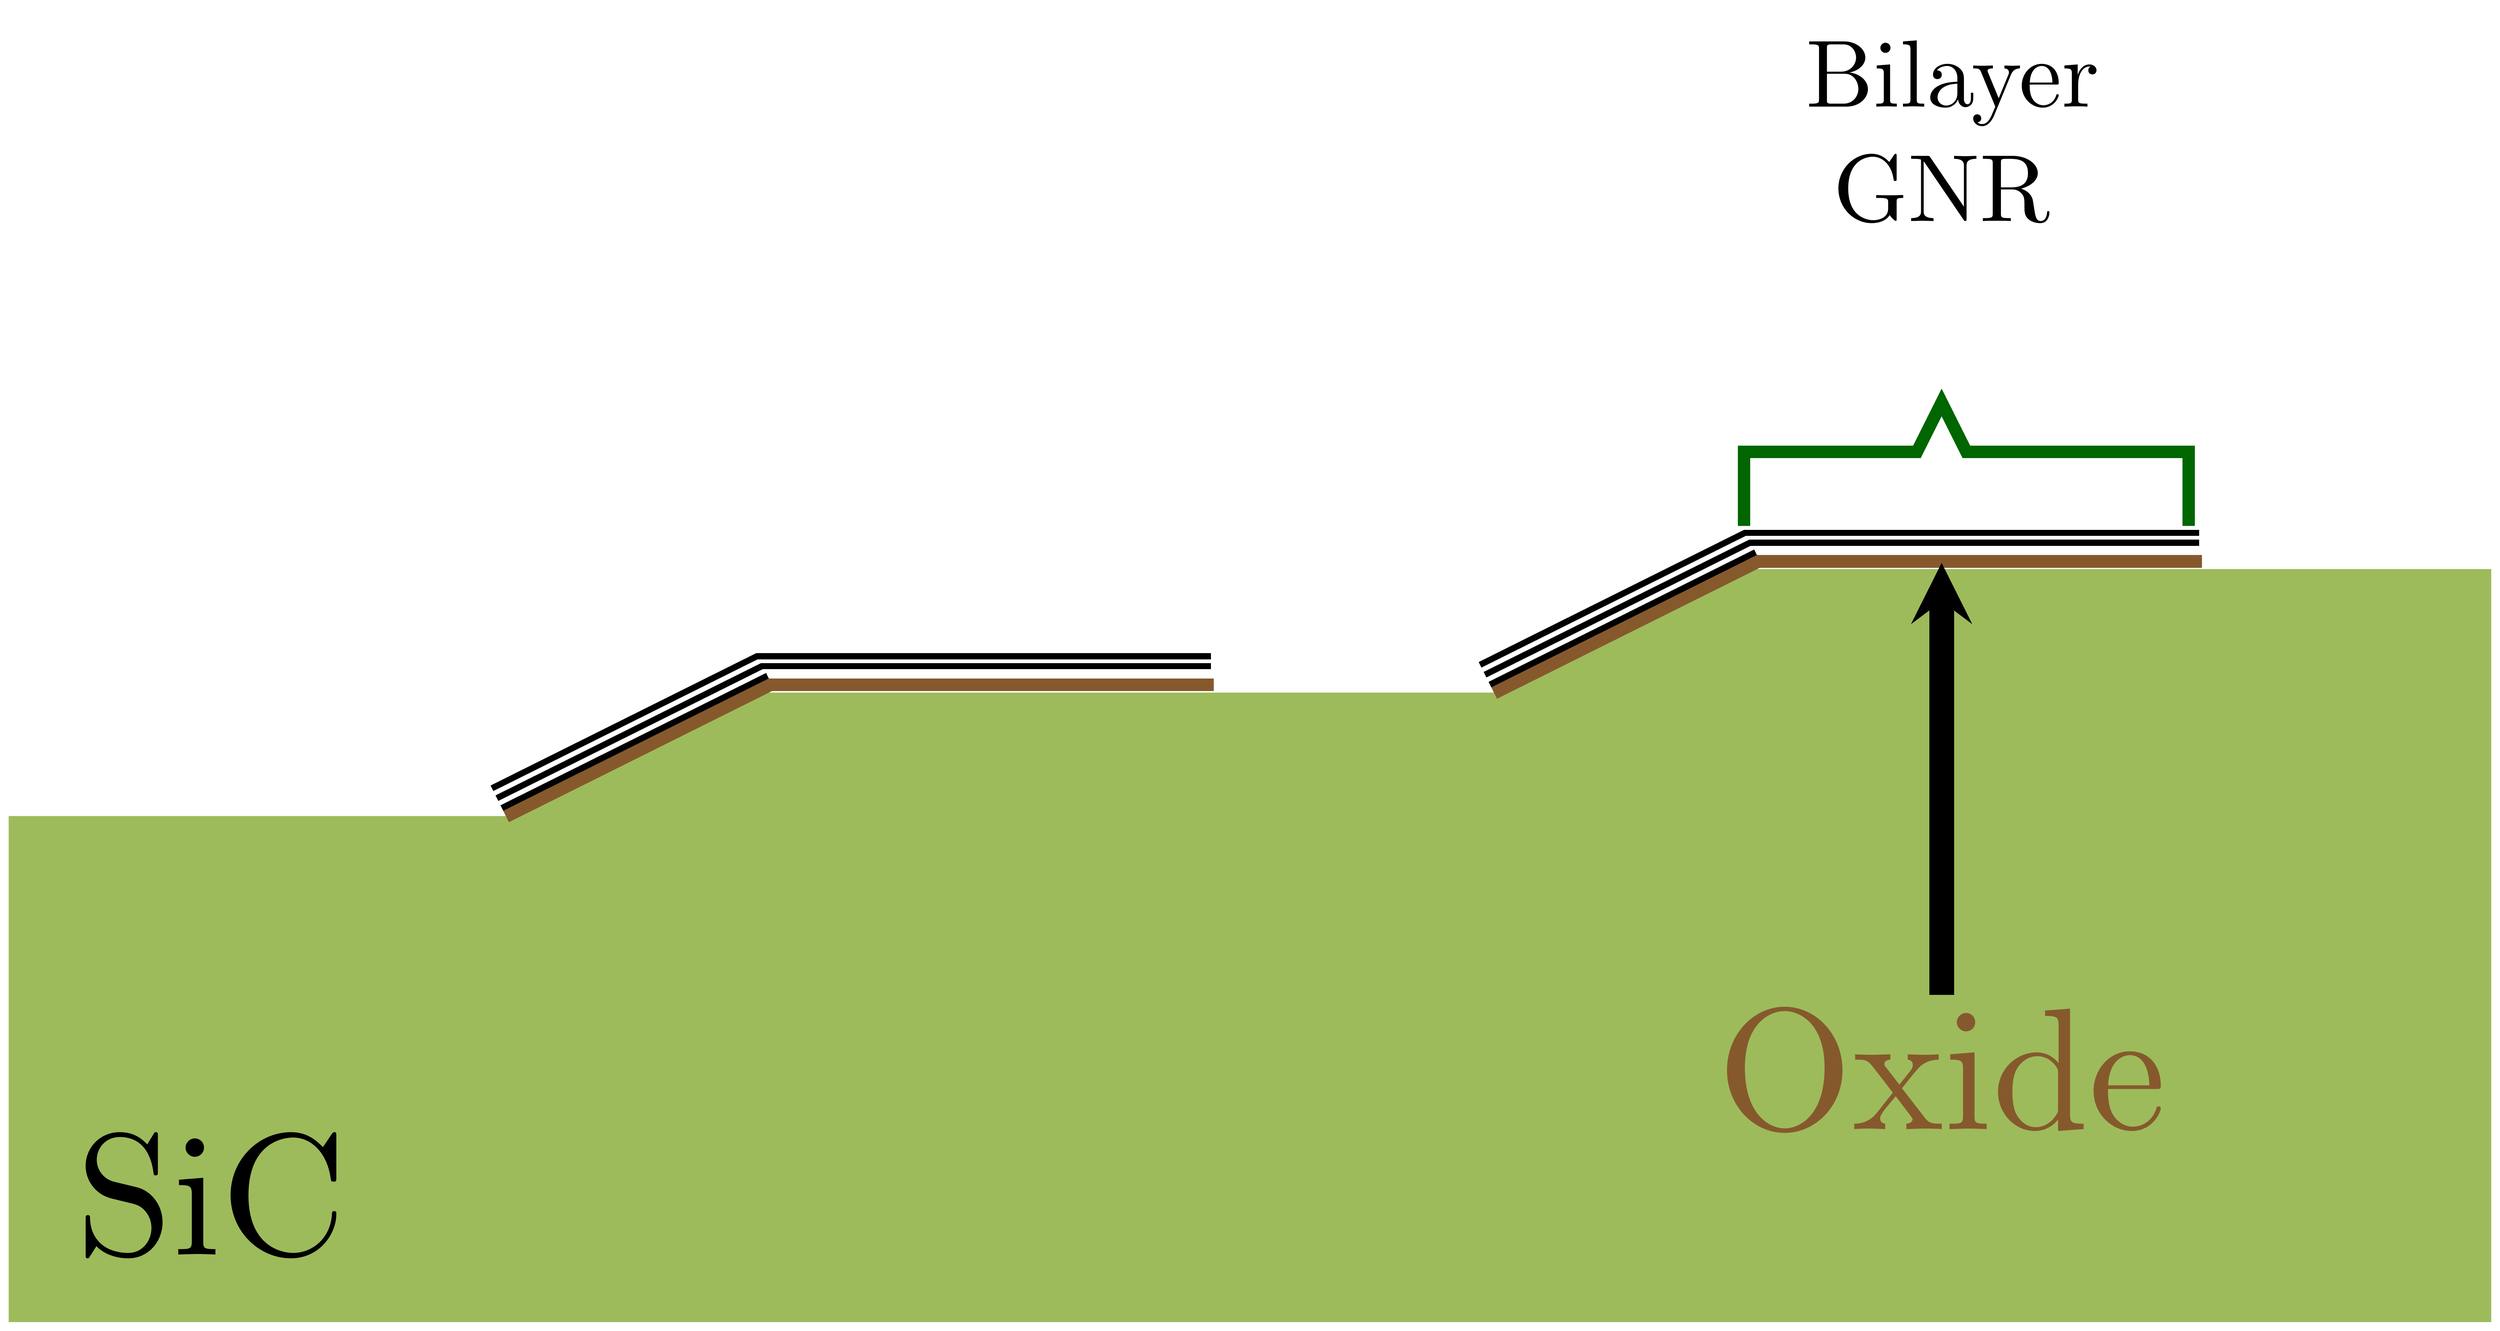
\begin{tikzpicture}[spy using outlines={circle,black, ultra thick,connect spies}]

\tikzset{>={Latex[width=15mm,length=15mm]}}

\draw[fill=limon,draw=limon,line width=5mm](0,0)--(100,0)--(100,30)--(70,30)--(60,25)--(30,25)--(20,20)--(0,20)--cycle;

\node[rotate=26.5,fill=brown!70!black]at (20,20) [draw=brown!70!black,name=e1ox1,rectangle, minimum width=120mm,minimum height=5mm,anchor=south west,transform shape] {};
\node[rotate=0,fill=brown!70!black]at (e1ox1.north east) [draw=brown!70!black,name=e1ox1c,rectangle, minimum width=180mm,minimum height=5mm,anchor=north west,transform shape] {};

\node[rotate=26.5,fill=black,yshift=0mm] at (e1ox1.north) [draw,name=e1l1,rectangle, minimum width=120mm,minimum height=1mm,anchor=south,transform shape] {};
\node[rotate=0,fill=black,yshift=0mm,opacity=0] at (e1l1.north east) [draw,name=e1lc,rectangle, minimum width=180mm,minimum height=1mm,anchor=north west,transform shape] {};

\node[rotate=26.5,fill=black,yshift=2mm] at (e1l1.north) [draw,name=e1l2,rectangle, minimum width=120mm,minimum height=1mm,anchor=south,transform shape] {};
\node[rotate=0,fill=black,yshift=0.mm] at (e1l2.north east) [draw,name=e1l2c,rectangle, minimum width=182mm,minimum height=1mm,anchor=north west,transform shape] {};

\node[rotate=26.5,fill=black,yshift=2mm] at (e1l2.north) [draw,name=e1l3,rectangle, minimum width=120mm,minimum height=1mm,anchor=south,transform shape] {};
\node[rotate=0,fill=black,yshift=0.mm] at (e1l3.north east) [draw,name=e1l3c,rectangle, minimum width=184mm,minimum height=1mm,anchor=north west,transform shape] {};

%===================================================================
\node[rotate=26.5,fill=,brown!70!black]at (60,25) [draw=,brown!70!black,name=e2ox1,rectangle, minimum width=120mm,minimum height=5mm,anchor=south west,transform shape] {};
\node[rotate=0,fill=,brown!70!black]at (e2ox1.north east) [draw=,brown!70!black,name=e2ox1c,rectangle, minimum width=180mm,minimum height=5mm,anchor=north west,transform shape] {};


\node[rotate=26.5,fill=black,yshift=0mm] at (e2ox1.north) [draw,name=e2l1,rectangle, minimum width=120mm,minimum height=1mm,anchor=south,transform shape] {};
\node[rotate=0,fill=black,yshift=0mm,opacity=0] at (e2l1.north east) [draw,name=e2lc,rectangle, minimum width=180mm,minimum height=1mm,anchor=north west,transform shape] {};


\node[rotate=26.5,fill=black,yshift=2mm] at (e2l1.north) [draw,name=e2l2,rectangle, minimum width=120mm,minimum height=1mm,anchor=south,transform shape] {};
\node[rotate=0,fill=black,yshift=0.mm] at (e2l2.north east) [draw,name=e2l2c,rectangle, minimum width=182mm,minimum height=1mm,anchor=north west,transform shape] {};

\node[rotate=26.5,fill=black,yshift=2mm] at (e2l2.north) [draw,name=e2l3,rectangle, minimum width=120mm,minimum height=1mm,anchor=south,transform shape] {};
\node[rotate=0,fill=black,yshift=0.mm] at (e2l3.north east) [draw,name=e2l3c,rectangle, minimum width=184mm,minimum height=1mm,anchor=north west,transform shape] {};


\draw[line width=5mm,green!40!black] (70,32)--(70,35)--(77,35)--(78,37)--(79,35)--(88,35)--(88,32);
\node[anchor=center, scale=11,text width=1cm,align=center] at (78,48) {Bilayer \\ GNR};
\node[anchor=center, scale=20,text width=1cm,align=center,brown!70!black](ox) at (78,10) {Oxide};
\draw[-{stealth},line width=10mm]([yshift=30mm]ox.center)--(78,30.5);

\node[anchor=south west,scale=20] at (0,0){SiC};
\end{tikzpicture}

\end{document}